\documentclass[12pt]{article}
\usepackage[utf8]{inputenc}

\usepackage{lmodern}

\usepackage{enumitem}
\usepackage[margin=2cm]{geometry}

\usepackage{amsmath, amsfonts, amssymb}
\usepackage{graphicx}
%\usepackage{subfigure}
\usepackage{tikz}
\usepackage{pgfplots}
\usepackage{multicol}

\usepackage{comment}
\usepackage{url}
\usepackage{calc}
\usepackage{subcaption}
\usepackage[indent=0pt]{parskip}
\usepackage{animate}

\usepackage{array}
\usepackage{blkarray,booktabs, bigstrut}
\usepackage{bigints}

\pgfplotsset{compat=1.16}

% MATH commands
\newcommand{\ga}{\left\langle}
\newcommand{\da}{\right\rangle}
\newcommand{\oa}{\left\lbrace}
\newcommand{\fa}{\right\rbrace}
\newcommand{\oc}{\left[}
\newcommand{\fc}{\right]}
\newcommand{\op}{\left(}
\newcommand{\fp}{\right)}

\newcommand{\bi}{\mathbf{i}}
\newcommand{\bj}{\mathbf{j}}
\newcommand{\bk}{\mathbf{k}}
\newcommand{\bF}{\mathbf{F}}

\newcommand{\mR}{\mathbb{R}}

\newcommand{\ra}{\rightarrow}
\newcommand{\Ra}{\Rightarrow}

\newcommand{\sech}{\mathrm{sech}\,}
\newcommand{\csch}{\mathrm{csch}\,}
\newcommand{\curl}{\mathrm{curl}\,}
\newcommand{\dive}{\mathrm{div}\,}

\newcommand{\ve}{\varepsilon}
\newcommand{\spc}{\vspace*{0.5cm}}

\DeclareMathOperator{\Ran}{Ran}
\DeclareMathOperator{\Dom}{Dom}

\newcommand{\exo}[1]{\noindent\textcolor{red}{\fbox{\textbf{Problem {#1}}}\hrulefill}\\}
\newcommand{\qu}[4]{\noindent\textcolor{#4}{\fbox{\textbf{Section {#1} | Problem {#2}}} \hrulefill{{\fbox{\textbf{{#3} Points}}}}\\}}

\newcommand{\semester}{Spring 2023}

\newcommand{\CVup}{%

\begin{tikzpicture}
\draw[black, <->, >=latex] (-0.33, 0.5) .. controls (-0.125, 0) and (0.125, 0) .. (0.33, 0.5);
\end{tikzpicture}}

\newcommand{\CVupInc}{%
\begin{tikzpicture}
\draw[black, ->, >=latex] (0,0) .. controls (0.2, 0) and (0.4, 0.2) .. (0.5, 0.5);
\end{tikzpicture}}

\newcommand{\CVupDec}{%
\begin{tikzpicture}[rotate=270]
\draw[black, ->, >=latex] (0,0) .. controls (0.2, 0) and (0.4, 0.2) .. (0.5, 0.5);
\end{tikzpicture}}

\newcommand{\CVdown}{%
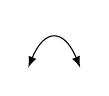
\begin{tikzpicture}
\draw[black, <->, >=latex] (-0.33, -0.5) .. controls (-0.125, 0) and (0.125, 0) .. (0.33, -0.5);
\end{tikzpicture}}

\newcommand{\CVdownInc}{%
\begin{tikzpicture}
\draw[black, ->, >=latex] (-0.5, -0.5) .. controls (-0.5, -0.3) and (-0.5, -0.1) .. (0,0);
\end{tikzpicture}}

\newcommand{\CVdownDec}{%
\begin{tikzpicture}[rotate=-90]
\draw[black, ->, >=latex] (-0.5, -0.5) .. controls (-0.5, -0.3) and (-0.5, -0.1) .. (0,0);
\end{tikzpicture}}

\begin{document}
	\noindent \hrulefill \\
	MATH-241 \hfill Pierre-Olivier Paris{\'e}\\
	Solutions Section 2-4 \hfill \semester \\\vspace*{-1cm}
	
	\noindent\hrulefill
	
	\spc
	
	\exo{1}
	\\
	Using the product rule, we have
		\begin{align*}
		f'(x) = (x^2)' \sin x + x^2 (\sin x)' = 2x \sin x + x^2 \cos (x) .
		\end{align*}
		
	\spc
	
	\exo{3}
	From the sum and difference rules, we have
		\begin{align*}
		f'(x) = 3 (\cot x)' - 2 (\cos x)' = -3 \csc^2 (x) + 2 \sin x .
		\end{align*}
	Notice that the negative sign became a plus sign because the derivative of $\cos x$ is $-\sin x$.
	
	\spc
	
	\exo{5}
	\\
	There are two ways to complete the problem.
		\begin{enumerate}
		\item We can use the product rule:
			\begin{align*}
			\frac{dy}{d\theta} &= \frac{d}{d\theta} (\sec \theta) \tan \theta + \sec \theta \frac{d}{d\theta} (\tan \theta ) \\
			&= \sec\theta \tan^2 \theta + \sec^3 \theta .
			\end{align*}
		\item We can rewrite the expression of $y$ as
			\begin{align*}
			y = \frac{1}{\cos \theta} \frac{\sin \theta}{\cos \theta} = \frac{\sin \theta}{\cos^2 \theta} .
			\end{align*}
		We then use the quotient rule:
			\begin{align*}
			y' &= \frac{\frac{d}{d\theta} (\sin \theta ) \cos^2 \theta - \sin \theta \frac{d}{d\theta} (\cos^2 \theta )}{\cos^4 \theta} \\
			&= \frac{\cos^3 \theta + 2 \sin^2 \theta \cos \theta}{\cos^4 \theta} \\
			&= \frac{\cos^2 \theta + 2 \sin^2 \theta}{\cos^3 \theta} .
			\end{align*}
		We can simplify further using $\sin^2 \theta + \cos^2 \theta = 1$ and then obtain
			\begin{align*}
			y' = \frac{\cos^2 + \sin^2 \theta + \sin^2 \theta}{\cos^3 \theta} = \frac{1 + \sin^2 \theta}{\cos^3 \theta} .
			\end{align*}
		\end{enumerate}
		
		\spc
		
	\exo{9}
	\\
	Using the quotient rule, we have
		\begin{align*}
		\frac{dy}{dx} &= \frac{1 (2 - \tan x) - x (-\sec^2 x)}{(2 - \tan x)^2} \\
		&= \frac{2 + x \sec^2 x - \tan x}{(2 - \tan x)^2} .
		\end{align*}
		
	\spc
	
	\exo{15}
	\\
	Using the product rule a first time:
		\begin{align*}
		f' (\theta ) = (\theta)' \cos \theta \sin \theta + \theta (\cos \theta \sin \theta )' .
		\end{align*}
	Using the product rule a second time:
		\begin{align*}
		(\cos \theta \sin \theta )' = -\sin^2 \theta + \cos^2 \theta = \cos (2\theta ) .
		\end{align*}
	Therefore, we get
		\begin{align*}
		f' (\theta) &= (1) \cos \theta \sin \theta + \theta \cos (2\theta ) \\
		&= \cos \theta \sin \theta + \theta \cos (2 \theta ) \\
		&= \tfrac{1}{2} \sin (2\theta ) + \theta \cos (2\theta ) .
		\end{align*}
	
\end{document}